% ENACT figure snippets for inline embedding in main.tex.

\begin{figure}[htbp]
\centering

\includegraphics[width=0.95\textwidth]{figures/fig1_pipeline.pdf}
\caption{ENACT pipeline schematic. (1) The $2\,\mu\mathrm{m}\times 2\,\mu\mathrm{m}$ bin-by-gene matrix from 10x Genomics Visium HD is ingested together with the paired full-resolution histology image. (2) Stardist segments cells in the tissue image. (3) Visium HD bins that intersect a cell outline are aggregated with one of four bin-to-cell assignment strategies (Naive or three weight-based variants). (4) Sargent, CellAssign or CellTypist translate per-cell transcript counts into cell-type labels. (5) Cell labels and coordinates are wrapped in AnnData objects compatible with Squidpy for neighbourhood enrichment, Moran's I, and co-occurrence analyses, and visualised with TissUUmaps.}
\label{fig:pipeline}
\end{figure}

\begin{figure}[htbp]
\centering
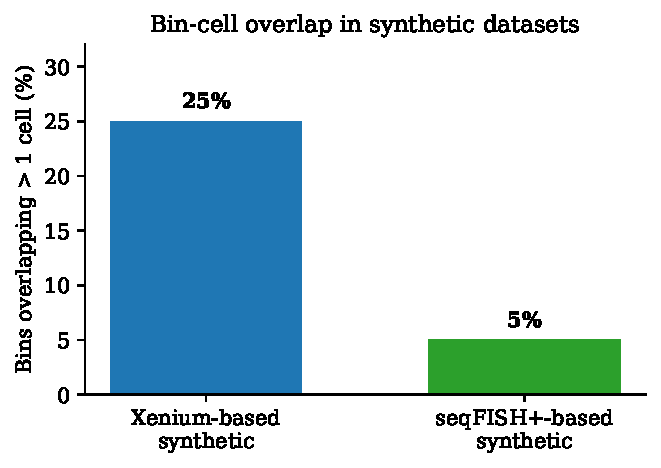
\includegraphics[width=0.55\textwidth]{figures/fig2_overlap.pdf}
\caption{Fraction of Visium HD bins that overlap more than one cell in the two synthetic datasets used for evaluation. On the Xenium-based synthetic dataset with whole-cell boundaries, about 25\% of bins overlap more than one cell, driving low recall for the Naive assignment strategy. On the seqFISH+-based synthetic dataset, only about 5\% of bins overlap more than one cell, so all four strategies perform comparably.}
\label{fig:overlap}
\end{figure}

\begin{figure}[htbp]
\centering
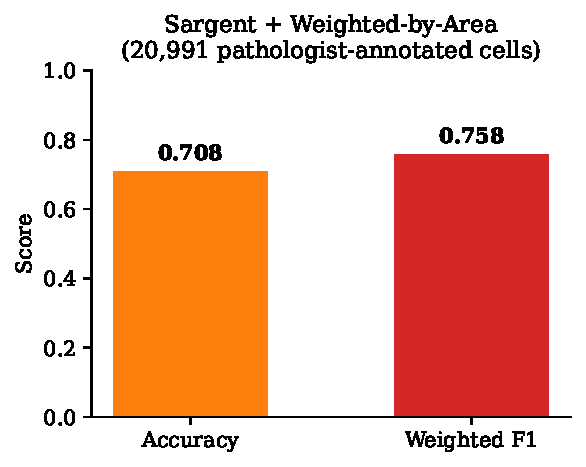
\includegraphics[width=0.55\textwidth]{figures/fig3_bestperf.pdf}
\caption{End-to-end cell-type classification performance of the best ENACT configuration (Sargent cell-type annotation combined with the Weighted-by-Area bin-to-cell assignment) on the cohort of 20{,}991 pathologist-annotated cells. The configuration reaches accuracy 0.708 and weighted F1 0.758.}
\label{fig:bestperf}
\end{figure}
